\documentclass[12pt, a4paper]{article}

% ─── Packages ─────────────────────────────────────────────────────────
\usepackage[utf8]{inputenc}
\usepackage[T1]{fontenc}
\usepackage{lmodern}
\usepackage[margin=2.5cm]{geometry}
\usepackage{graphicx}
\usepackage{booktabs}
\usepackage{longtable}
\usepackage{hyperref}
\usepackage{caption}
\usepackage{subcaption}
\usepackage{amsmath}
\usepackage{enumitem}
\usepackage{xcolor}
\usepackage{float}
\usepackage{natbib}
\usepackage{setspace}
\usepackage{tikz}
\usetikzlibrary{arrows.meta, positioning, shapes.geometric, fit}

\hypersetup{
    colorlinks=true,
    linkcolor=blue!70!black,
    citecolor=green!50!black,
    urlcolor=blue!60!black,
}

\onehalfspacing
\graphicspath{{figures/}}

\title{%
  \vspace{-1.5cm}
  \textbf{Named Entity Recognition in Football Journalism:\\
  A Comparative Analysis of Men's and Women's Coverage}
}
\author{Ziv}
\date{February 2026}

\begin{document}

\maketitle

\begin{abstract}
This report presents a comprehensive Named Entity Recognition (NER) pipeline applied to football journalism, with the goal of testing fifteen hypotheses about entity prominence, club co-occurrence, and gendered framing differences between men's and women's football coverage. Our data pipeline combines web scraping from four independent sources (GDELT, BBC RSS, direct site crawling, and dedicated women's football outlets) with seven Kaggle football datasets, yielding a combined corpus of over 20,000 unique articles. After cleaning, deduplication, football-relevance filtering, and gender classification, we retain 11,386 men's and 563 women's articles from Kaggle, supplemented by 2,316 scraped women's articles to address class imbalance. We evaluate three spaCy NER models on the SocCor UEFA EURO~2024 corpus (121 documents, 13,353 gold player mentions) and select \texttt{en\_core\_web\_lg} (F1\,=\,0.812) as our primary model. Detailed error analysis reveals that 40.4\% of shared model blind spots involve single-word surname references, and players from Eastern/Central European countries are disproportionately missed. Through gazetteer-enhanced entity classification and context-window hypothesis testing with formal statistical tests (Mann-Whitney U, Chi-square, proportion z-tests) and effect-size reporting (Cohen's~$d$, Cram\'er's~$V$, Cohen's~$h$), we find strong evidence for gendered differences in naming conventions (H10), meta-discourse about league growth (H14), and attribute framing (H12), alongside classical NER results confirming Zipfian player prominence (H1) and transfer-window MONEY spikes (H4). All $p$-values are corrected for multiple comparisons using Benjamini-Hochberg FDR adjustment.
\end{abstract}

\tableofcontents
\newpage

% ═══════════════════════════════════════════════════════════════════════
\section{Introduction}
\label{sec:intro}
% ═══════════════════════════════════════════════════════════════════════

Named Entity Recognition is a fundamental NLP task that identifies real-world referents---persons, organisations, locations---in unstructured text. In the football domain, accurate NER enables downstream analyses such as player prominence tracking, club co-occurrence network construction, and gendered framing analysis.

This project addresses two overarching research questions:
\begin{enumerate}[label=\textbf{RQ\arabic*.}]
    \item What structural patterns emerge from entity distributions in football journalism (e.g., player prominence, club clustering, transfer windows)?
    \item How does the \emph{framing} of entities differ between men's and women's football coverage in terms of naming conventions, descriptive language, and meta-discourse?
\end{enumerate}

We operationalise these questions through fifteen testable hypotheses grouped into \textbf{core football} (H1--H5) and \textbf{men vs.\ women portrayal} (H9--H16), plus a diagnostic analysis (D1) on entity diversity.


% ═══════════════════════════════════════════════════════════════════════
\section{Data Sources}
\label{sec:data}
% ═══════════════════════════════════════════════════════════════════════

Our data comes from two broad categories: (1)~pre-existing Kaggle datasets covering general football journalism using which we run the hypothesis analysis, and (2)~a purpose-built web-scraping pipeline targeting Champions League and women's football coverage. Additionally, we use the SocCor corpus as ground truth for NER evaluation.

% ──────────────────────────────────────────────────────────────────────
\subsection{Source 1: Kaggle Football Datasets}
\label{sec:kaggle}
% ──────────────────────────────────────────────────────────────────────

We aggregated seven CSV files from the \texttt{data/kaggle\_data\_football/} directory, each with a different schema (Table~\ref{tab:kaggle_sources}).

\begin{table}[H]
\centering
\caption{Kaggle data sources and article counts.}
\label{tab:kaggle_sources}
\small
\begin{tabular}{lrll}
\toprule
\textbf{File} & \textbf{Raw rows} & \textbf{Primary source} & \textbf{Coverage} \\
\midrule
\texttt{final-articles.csv}    & 11,963 & Goal.com, multi-source & General football \\
\texttt{goal-news.csv}         &  7,596 & Goal.com                & News, match reports \\
\texttt{df\_analyst.csv}       &  1,960 & The Analyst              & Analytics, reviews \\
\texttt{tribuna\_articles.csv} &  1,500 & Tribuna.com              & Fan community \\
\texttt{allfootball.csv}       &    800 & All Football App         & Mixed \\
\texttt{skysports.csv}         &    278 & Sky Sports               & Premier League focus \\
\texttt{live\_mint.csv}        &     40 & LiveMint                 & Indian perspective \\
\midrule
\textbf{Total (raw)}           & 24,137 & & \\
\bottomrule
\end{tabular}
\end{table}

% ──────────────────────────────────────────────────────────────────────
\subsection{Source 2: Web Scraping Pipeline}
\label{sec:scraping}
% ──────────────────────────────────────────────────────────────────────

To supplement the Kaggle data---particularly for women's football, which is under-represented in general datasets---we built a four-stage scraping pipeline, orchestrated by \texttt{run\_all\_scrapers.py} and configured centrally via \texttt{config.py}.

\subsubsection{Stage A: GDELT API Scraping (\texttt{1\_scrape\_gdelt.py})}

The GDELT DOC~2.0 API was queried using sliding 60-day date windows from January 2023 to February 2026. For \textbf{men's coverage}, 15 queries targeted Champions League content (e.g., \texttt{"Champions League" match report football}, \texttt{"Champions League" football transfer}). For \textbf{women's coverage}, 37 queries spanned UWCL, WSL, Liga~F, NWSL, Women's World Cup, and individual club teams (e.g., \texttt{"Women's Champions League" football}, \texttt{"WSL" football match report}, \texttt{"Barcelona Femeni" football}, \texttt{"Lionesses" football England women}).

Each GDELT query returns up to 250 article URLs. Full article text was then extracted using Trafilatura with concurrent thread-pool downloading (6 workers), respecting rate limits of 2\,s between GDELT queries and 1\,s between Trafilatura fetches. Blocked domains (e.g., Irish regional newspapers returning non-football content) were filtered out. Articles were saved as individual JSON files with metadata including URL, title, date, domain, source country, language, and word count.

\textbf{Result:} 11,547 men's and 14,712 women's raw JSON articles.

\subsubsection{Stage B: BBC Sport RSS (\texttt{2\_scrape\_bbc\_rss.py})}

BBC Sport RSS feeds were parsed for Champions League, European Championship (men's), and Women's Football sections. For each entry, Trafilatura extracted the full article body. Articles shorter than 50 words were discarded. Duplicate URLs were tracked across runs to avoid re-downloading.

\textbf{Result:} 65 men's and 34 women's articles.

\subsubsection{Stage C: Direct Website Crawling (\texttt{3\_scrape\_web\_direct.py})}

Seed URLs from UEFA.com (UCL and UWCL news pages) and Goal.com (Champions League and women's football sections) were crawled to discover article links matching domain-specific URL patterns. Discovered URLs were then processed through Trafilatura for full-text extraction.

\textbf{Result:} 11 men's and 14 women's articles.

\subsubsection{Stage D: Expanded Women's Scraping (\texttt{6\_scrape\_women\_expanded.py})}

Recognising the persistent class imbalance, an expanded women's football scraper targeted additional sources: BBC Sport Women's Football (sitemap/archive discovery), SkySports Women's Football news pages, re-queried GDELT with simpler terms to catch previously missed articles, and Trafilatura's sitemap discovery for known women's football domains. This scraper maintained a shared URL deduplication set across all women's source directories.


% ──────────────────────────────────────────────────────────────────────
\subsection{Source 3: SocCor UEFA EURO 2024 Corpus}
\label{sec:soccor_data}
% ──────────────────────────────────────────────────────────────────────

The \textbf{SocCor} corpus is a multilingual football commentary corpus annotated with inline player tags of the form \texttt{<SURNAME\_POSITION\_COUNTRY>} (e.g., \texttt{<BELLINGHAM\_ATTACKING-MIDFIELD\_ENG>}). We use the \textbf{English BBC} subset (121 documents, 13,353 gold player mentions) as ground truth for NER model evaluation. The corpus spans match reports, live game commentaries, highlights, and livetickers from the UEFA EURO 2024 tournament.

SocCor also provides metadata:
\begin{itemize}[nosep]
    \item \texttt{Players.csv}: 646 players with full name, token mapping, position, club, and market value.
    \item \texttt{Groups.csv}: Participating national teams grouped by tournament stage.
    \item \texttt{Broadcasters.csv}: Media outlets per country.
\end{itemize}


% ═══════════════════════════════════════════════════════════════════════
\section{Data Processing Pipeline}
\label{sec:pipeline}
% ═══════════════════════════════════════════════════════════════════════

The processing pipeline consists of seven stages, implemented as standalone scripts.

% ──────────────────────────────────────────────────────────────────────
\subsection{Stage 1: Scraped Data Cleaning and Merging}
\label{sec:clean_merge}
% ──────────────────────────────────────────────────────────────────────

\textbf{Script:} \texttt{5\_clean\_and\_merge.py}

All raw scraped JSON files from every source subdirectory (\texttt{gdelt/}, \texttt{bbc/}, \texttt{web\_scraped/}) were loaded and merged per gender category. The cleaning pipeline applied three text transformations in sequence:

\begin{enumerate}[nosep]
    \item \textbf{HTML stripping:} Residual HTML tags were removed using BeautifulSoup with a regex fallback.
    \item \textbf{Encoding repair:} Common mojibake artefacts (e.g., \texttt{\textbackslash u00e2\textbackslash u0080\textbackslash u0099}~$\rightarrow$~apostrophe, non-breaking spaces~$\rightarrow$~regular spaces) were corrected, followed by Unicode NFC normalisation.
    \item \textbf{Whitespace normalisation:} Multiple consecutive whitespace characters were collapsed into single spaces.
\end{enumerate}

Articles with fewer than 50 words were discarded. Three-stage deduplication then removed duplicates by: (1)~exact URL match, (2)~case-insensitive title match, and (3)~near-duplicate body text (first 200 characters match).

\textbf{Result:} 6,585 men's and 2,316 women's cleaned, deduplicated scraped articles, saved to \texttt{data/final\_processed/}.


% ──────────────────────────────────────────────────────────────────────
\subsection{Stage 2: Kaggle Schema Normalisation and Deduplication}
\label{sec:stage2}
% ──────────────────────────────────────────────────────────────────────

\textbf{Script:} \texttt{classify\_kaggle.py}

Each of the seven Kaggle CSVs has a different column schema. Per-file column mappings normalised all data into a unified schema: \texttt{article\_id | title | body\_text | link | author | publish\_time | source}. Missing columns were filled with empty strings. Deduplication on \texttt{(title, link)} removed 11,970 duplicate rows (largely overlapping articles between \texttt{final-articles.csv} and \texttt{goal-news.csv}). Articles with fewer than 50 characters of body text were discarded.

\textbf{Result:} 24,137 raw $\rightarrow$ 12,167 deduplicated $\rightarrow$ \textbf{11,949 final Kaggle articles}.


% ──────────────────────────────────────────────────────────────────────
\subsection{Stage 3: Gender Classification}
\label{sec:gender_class}
% ──────────────────────────────────────────────────────────────────────

Since no ground-truth gender labels exist in the Kaggle data, we applied \textbf{keyword-based classification} using a compiled regular expression with 40+ patterns:

\begin{itemize}[nosep]
    \item \textbf{Direct indicators:} \texttt{women's football}, \texttt{WSL}, \texttt{NWSL}, \texttt{UWCL}, \texttt{Liga~F}, etc.
    \item \textbf{Team names:} \texttt{Lionesses}, \texttt{USWNT}, \texttt{Matildas}, \texttt{Banyana Banyana}, etc.
    \item \textbf{Club variants:} \texttt{Chelsea Women}, \texttt{Barcelona Femen\'i}, \texttt{Arsenal Women}, etc.
    \item \textbf{Competition names:} \texttt{She Believes Cup}, \texttt{Arnold Clark Cup}, \texttt{Women's World Cup}, etc.
\end{itemize}

Both \texttt{title} and \texttt{body\_text} were searched. An article was labelled \textit{women} if any pattern matched; otherwise \textit{other} (predominantly men's).

\textbf{Result:} \textbf{Women's:} 563 articles (4.7\%), \textbf{Other (men's):} 11,386 articles (95.3\%).


% ──────────────────────────────────────────────────────────────────────
\subsection{Stage 4: Final Input Assembly}
\label{sec:final_input}
% ──────────────────────────────────────────────────────────────────────

\textbf{Script:} \texttt{prepare\_final\_inputs.py}

Given the severe class imbalance in the Kaggle data (563 women's vs.\ 11,386 men's), we combined the Kaggle women's articles with the cleaned scraped women's articles (\S\ref{sec:clean_merge}) to create a larger women's corpus. Schema normalisation mapped the scraped columns (\texttt{url}, \texttt{domain}, \texttt{date}) to the Kaggle schema (\texttt{link}, \texttt{source}, \texttt{publish\_time}). Title-based deduplication between the two sources ensured no overlap.

For men's articles, \textbf{only the Kaggle data} was used in the final analysis. While the scraping pipeline successfully collected 6,585 men's articles, computational resource constraints (NER processing time and memory) prevented us from running the full pipeline on the combined corpus. The scraped men's data is available for future analysis.

\textbf{Final corpus for NER analysis:}
\begin{itemize}[nosep]
    \item \textbf{Men's/Other:} 11,386 articles (Kaggle only)
    \item \textbf{Women's:} Kaggle (563) + scraped (2,316) = combined corpus (after deduplication)
\end{itemize}


% ──────────────────────────────────────────────────────────────────────
\subsection{Stage 5: NER Model Evaluation on SocCor}
\label{sec:soccor_eval}
% ──────────────────────────────────────────────────────────────────────

\textbf{Script:} \texttt{8b\_evaluate\_soccor.py}

Before running NER on our corpus, we evaluated model accuracy using SocCor as ground truth. Figure~\ref{fig:soccor_pipeline} illustrates the evaluation pipeline.

\begin{figure}[H]
\centering
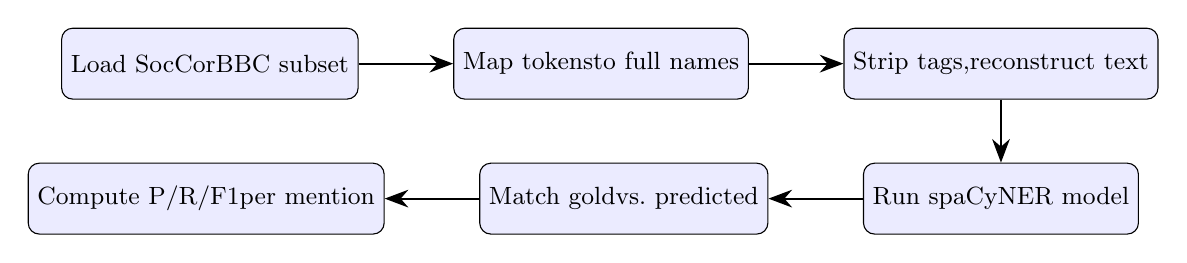
\begin{tikzpicture}[
    node distance=0.8cm and 1.2cm,
    block/.style={rectangle, draw, rounded corners, minimum width=2.8cm, minimum height=0.9cm, text centered, font=\small, fill=blue!8},
    decision/.style={diamond, draw, aspect=2.5, font=\small, fill=orange!10, inner sep=1pt},
    arrow/.style={-{Stealth[length=3mm]}, thick},
]
    \node[block] (load) {Load SocCor\\BBC subset};
    \node[block, right=of load] (meta) {Map tokens\\to full names};
    \node[block, right=of meta] (strip) {Strip tags,\\reconstruct text};
    \node[block, below=of strip] (ner) {Run spaCy\\NER model};
    \node[block, left=of ner] (match) {Match gold\\vs.\ predicted};
    \node[block, left=of match] (metrics) {Compute P/R/F1\\per mention};

    \draw[arrow] (load) -- (meta);
    \draw[arrow] (meta) -- (strip);
    \draw[arrow] (strip) -- (ner);
    \draw[arrow] (ner) -- (match);
    \draw[arrow] (match) -- (metrics);
\end{tikzpicture}
\caption{SocCor NER evaluation pipeline. Inline tags are replaced with full player names from \texttt{Players.csv}, then spaCy predictions are matched against gold entities using exact name, surname, or substring containment.}
\label{fig:soccor_pipeline}
\end{figure}

The pipeline operates as follows:
\begin{enumerate}[nosep]
    \item \textbf{Token-to-name mapping:} \texttt{Players.csv} (646 entries) maps inline tags to full player names (e.g., \texttt{<STEGEN\_GOALKEEPER\_GER>}~$\rightarrow$~``Marc-Andr\'e ter Stegen'' instead of the fallback ``Stegen'').
    \item \textbf{Text reconstruction:} Inline tags are stripped and replaced with the mapped full name, producing clean text suitable for NER.
    \item \textbf{NER execution:} Each spaCy model processes the clean text, extracting all \texttt{PERSON}-labelled entities.
    \item \textbf{Matching:} For each gold entity, we check whether any spaCy \texttt{PERSON} entity matches by: (a)~exact full name, (b)~mutual substring containment, (c)~surname match, or (d)~individual name-part match.
    \item \textbf{Metrics:} Precision (\textit{what fraction of spaCy PERSON predictions are real players}), recall (\textit{what fraction of gold players were detected}), and F1 are computed at the mention level.
\end{enumerate}

\begin{table}[H]
\centering
\caption{SocCor NER evaluation results (121 BBC documents, 13,353 gold player mentions).}
\label{tab:soccor_eval}
\begin{tabular}{lcccrrr}
\toprule
\textbf{Model} & \textbf{Precision} & \textbf{Recall} & \textbf{F1} & \textbf{TP} & \textbf{FN} & \textbf{FP} \\
\midrule
\texttt{en\_core\_web\_sm} & 0.749 & 0.758 & 0.754 & 10,127 & 3,226 & 3,389 \\
\texttt{en\_core\_web\_lg} & 0.754 & \textbf{0.880} & \textbf{0.812} & 11,749 & 1,604 & 3,832 \\
\bottomrule
\end{tabular}
\end{table}

\noindent\textbf{Decision:} \texttt{en\_core\_web\_lg} was selected as the primary model, offering +7.6\% F1 and +12.2\% recall over \texttt{en\_core\_web\_sm}. Its substantially higher recall (0.880 vs.\ 0.758) was particularly important for our downstream analysis, which relies on detecting as many player mentions as possible.


% ──────────────────────────────────────────────────────────────────────
\subsection{Stage 5a: SocCor Error Analysis}
\label{sec:error_analysis}
% ──────────────────────────────────────────────────────────────────────

\textbf{Script:} \texttt{8c\_soccor\_error\_analysis.py}

To understand \textit{where} and \textit{why} the NER models fail, we conducted a detailed error analysis that recorded every individual false negative (missed player) and false positive (spurious detection) with full context.

\paragraph{Most-missed players.}
Table~\ref{tab:top_missed} shows the players most frequently missed by each model. Mbapp\'e is the single most-missed player (262 times by \texttt{sm}, 209 by \texttt{lg}), primarily because his name appears in live commentary as a bare surname---a pattern that spaCy's general English models struggle with for non-English names.

\begin{table}[H]
\centering
\caption{Top-5 most frequently missed players by each model.}
\label{tab:top_missed}
\small
\begin{tabular}{llrrr}
\toprule
\textbf{Player} & \textbf{Country} & \textbf{Position} & \textbf{sm misses} & \textbf{lg misses} \\
\midrule
Mbapp\'e            & FRA & Centre Forward   & 262 & 209 \\
Hernandez           & FRA & Left Back        & 132 & --- \\
Demb\'el\'e         & FRA & Right Winger     & 119 & --- \\
Denzel Dumfries     & NED & Right Midfield   & 102 & 102 \\
Kound\'e            & FRA & Centre Back      &  77 &  42 \\
Memphis Depay       & NED & Centre Forward   &  42 &  63 \\
Lamine Yamal       & ESP & Right Winger     & --- &  57 \\
\bottomrule
\end{tabular}
\end{table}

\paragraph{Shared blind spots.}
451 mention-level instances were missed by \textit{both} models. Pattern analysis revealed:
\begin{itemize}[nosep]
    \item \textbf{40.4\% are single-word surnames} (e.g., ``Mbapp\'e'', ``Kant\'e'', ``Kound\'e''): spaCy struggles with bare surnames lacking a preceding first name, especially for non-English names with diacritics.
    \item \textbf{27.9\% are Eastern/Central European players} (Turkey, Romania, Georgia, Slovakia, etc.): names with unfamiliar morphology for English-trained models (e.g., Bar{\i}\c{s} Alper Y{\i}lmaz, Milan \v{S}kriniar).
    \item \textbf{Centre backs are disproportionately missed} (121 of 451 shared misses): defenders' surnames are commonly used without first names in rapid live commentary.
\end{itemize}

\paragraph{Document type matters.}
Games/live commentary text accounts for \textbf{93.6\%} of all false negatives (3,019/3,226 for \texttt{sm}; 1,466/1,604 for \texttt{lg}). This is because live commentary uses informal, rapid-fire surname-only references (``Mbapp\'e drives forward'') far more than match reports, which tend to introduce players by full name.

\paragraph{Common false positives.}
The most frequent spurious \texttt{PERSON} detections included: ``Euros'' (96 times by \texttt{sm}---a tournament name misclassified), ``Pepe'' and ``Mudrik'' (real players but not in the gold annotation set for the specific document), ``Austria'' (country name misclassified), ``Goal'' (common noun), and referee names like ``Anthony Taylor'' and ``Michael Oliver'' (correctly \texttt{PERSON} but not in the gold \textit{player} set).


% ──────────────────────────────────────────────────────────────────────
\subsection{Stage 6: NER Extraction with Gazetteer Enhancement}
\label{sec:ner_pipeline}
% ──────────────────────────────────────────────────────────────────────

\textbf{Script:} \texttt{7\_run\_ner.py}

The NER pipeline processes each article through a carefully designed classification cascade:

\begin{enumerate}[nosep]
    \item \textbf{Football relevance filtering:} Each article is checked against 100+ domain keywords (e.g., ``goal'', ``transfer'', ``league'', ``penalty'', ``offside''). Articles matching fewer than 3 keywords are classified as non-football and skipped. Additionally, articles containing American sports terms (``touchdown'', ``quarterback'', ``inning'') are rejected.
    \item \textbf{SpaCy NER:} \texttt{en\_core\_web\_lg} extracts all named entities from the article body (truncated to 10,000 characters for memory safety). The \texttt{tagger}, \texttt{parser}, and \texttt{lemmatizer} components are disabled for speed, processing articles in batches of 100 via \texttt{nlp.pipe()}.
    \item \textbf{Domain-specific reclassification:} Each spaCy entity passes through a priority cascade:
    \begin{enumerate}[nosep, label=\alph*)]
        \item \textbf{Noise filter:} Non-football entities (``Trump'', ``NFL'', ``Tesla'', etc.---a curated list of 35+ terms) are removed entirely.
        \item \textbf{Gazetteer matching:} Entity text is normalised (lowercase, quote stripping, article removal, whitespace collapse) and checked against five separate gazetteers in priority order:
        \begin{itemize}[nosep]
            \item \textsc{Competition} (40+ entries): ``Champions League'', ``WSL'', ``Copa del Rey'', etc.
            \item \textsc{Media} (35+ entries): ``Sky Sports'', ``BBC Sport'', ``ESPN'', etc.
            \item \textsc{Club} (130+ static entries + 219 from SocCor \texttt{Players.csv} club column): ``Chelsea'', ``Barcelona'', ``Portland Thorns'', etc.
            \item \textsc{Governing Body} (20+ entries): ``FIFA'', ``UEFA'', ``The FA'', etc.
            \item \textsc{Player} (1,279 entries from SocCor \texttt{Players.csv}---full names + surnames): ``Florian Wirtz'', ``Wirtz'', ``Mbapp\'e'', etc.
        \end{itemize}
        \item \textbf{SpaCy-label fallback:} Unmatched entities use their spaCy label (e.g., \texttt{PERSON}~$\rightarrow$~\textsc{Player}, \texttt{ORG}~$\rightarrow$~\textsc{Org\_Other}, \texttt{GPE}~$\rightarrow$~\textsc{Location}, \texttt{MONEY}~$\rightarrow$~\textsc{Money}).
    \end{enumerate}
    \item \textbf{Context capture:} For each entity, a $\pm$50-character window around the mention is saved as \texttt{sentence\_context}, enabling downstream hypothesis testing on the language \textit{surrounding} entity mentions.
\end{enumerate}

\noindent\textbf{Key design decision:} The \textsc{Player} gazetteer (from \texttt{Players.csv}) is kept \textbf{completely separate} from the \textsc{Club} gazetteer. Player names (1,279 normalised entries) and club names (130+ static + 219 from the club column) never overlap, preventing misclassification of players with club-like names.

\noindent\textbf{Result:}
\begin{itemize}[nosep]
    \item \textbf{Other (men's):} 37,089 entities from 718 articles (9,652 unique); 282 articles filtered as non-football
    \item \textbf{Women's:} 24,464 entities from 369 articles (7,050 unique); 194 articles filtered as non-football
\end{itemize}

\begin{figure}[H]
    \centering
    \includegraphics[width=\textwidth]{summary_entity_distribution.png}
    \caption{Entity label distribution comparison between men's and women's coverage. The \textsc{Player} label dominates both, but men's shows a higher proportion of \textsc{Player} mentions relative to other entity types.}
    \label{fig:entity_dist}
\end{figure}


% ═══════════════════════════════════════════════════════════════════════
\section{Hypotheses}
\label{sec:hypotheses}
% ═══════════════════════════════════════════════════════════════════════

\subsection{A. Core Football Entity-Occurrence Hypotheses}

These hypotheses examine structural patterns in entity distributions, testable via NER counts and co-occurrence analysis.

\begin{description}[style=nextline, leftmargin=1.2cm]
    \item[\textbf{H1.}] \textbf{Prominence.} A small number of \textsc{Player} entities dominate mentions within each category, following a heavy-tail Zipfian distribution (e.g., the top-10 players account for a disproportionate share of mentions).

    \item[\textbf{H2.}] \textbf{Club centrality.} \textsc{Club} co-occurrence networks form distinct clusters by competition (domestic league vs.\ continental tournament), and the purity of these clusters differs between men's and women's coverage.

    \item[\textbf{H3.}] \textbf{Manager-focus.} In articles with manager/coach mentions, negative event terms (``sacked'', ``under pressure'', ``crisis'') co-occur more frequently, and the rate of such co-occurrence differs between men's and women's coverage.

    \item[\textbf{H4.}] \textbf{Transfer windows.} In transfer-related articles, \textsc{Player}\,$\leftrightarrow$\,\textsc{Club} co-occurrences increase sharply and \textsc{Money} mentions spike, with measurable effect sizes.

    \item[\textbf{H5.}] \textbf{Injury narrative.} Articles exhibit a rich injury/fatigue vocabulary; women's coverage may show different injury patterns (particularly ACL-related terms) compared to men's.
\end{description}

\subsection{B. Men vs.\ Women Portrayal Hypotheses}

These hypotheses examine \emph{how} entities are framed differently, testable via context-window analysis around entity mentions.

\begin{description}[style=nextline, leftmargin=1.5cm]
    \item[\textbf{H9.}] \textbf{Individual vs.\ team emphasis.} Women's reports contain fewer distinct \textsc{Player} entities per article and a different player-to-club ratio compared to men's.

    \item[\textbf{H10.}] \textbf{Name formality.} Women's articles use full names (first + last) for \textsc{Player} at a higher rate; men's articles use surname-only at a higher rate.

    \item[\textbf{H11.}] \textbf{Role framing.} Women's articles mention youth/age descriptors near \textsc{Player} more often; men's mention experience/legacy terms more often.

    \item[\textbf{H12.}] \textbf{Attribute mix.} Women's coverage uses more mentality/effort descriptors (``brave'', ``determined'') near \textsc{Player}; men's uses more physicality/tactical descriptors (``powerful'', ``clinical'').

    \item[\textbf{H13.}] \textbf{Relational framing.} Women's coverage includes more relational mentions near \textsc{Player} (``captain'', ``teammate'') than men's, which favours ``star'' framing.

    \item[\textbf{H14.}] \textbf{Meta-discourse.} Women's coverage contains more ``league growth / visibility / professionalisation'' terms co-occurring with \textsc{Competition}/\textsc{Club}.

    \item[\textbf{H15.}] \textbf{Credit assignment.} In win-related articles, men's reports attribute success to individual \textsc{Player} entities more often; women's reports credit the collective.

    \item[\textbf{H16.}] \textbf{Source framing bias.} Different news outlets (Goal.com, The Analyst, Tribuna, etc.) exhibit different entity framing patterns, measurable via Kruskal-Wallis tests across sources.
\end{description}

\subsection{C. Diagnostic Analysis}

\begin{description}[style=nextline, leftmargin=1.2cm]
    \item[\textbf{D1.}] \textbf{Entity diversity.} Shannon entropy of entity label distributions per article differs between men's and women's coverage, reflecting differences in coverage breadth.
\end{description}


% ═══════════════════════════════════════════════════════════════════════
\section{Methodology}
\label{sec:methodology}
% ═══════════════════════════════════════════════════════════════════════

All hypothesis testing is implemented in \texttt{10\_hypothesis\_analysis.py}. The general approach combines context-window linguistic analysis with formal statistical testing.

\subsection{Analysis Framework}

For each hypothesis, we follow a five-step procedure:
\begin{enumerate}[nosep]
    \item \textbf{Entity selection:} Filter entities by label (e.g., \textsc{Player}, \textsc{Club}, \textsc{Competition}).
    \item \textbf{Context-window analysis:} Search the $\pm$50-character \texttt{sentence\_context} around each entity for hypothesis-specific keyword patterns, compiled as case-insensitive word-boundary regular expressions.
    \item \textbf{Aggregation:} Compute per-article or per-entity rates, then compare between \textit{men's} and \textit{women's} categories.
    \item \textbf{Statistical testing:} Apply appropriate tests depending on data type:
    \begin{itemize}[nosep]
        \item \textbf{Mann-Whitney U} for comparing continuous distributions between two groups (player counts, term rates).
        \item \textbf{Chi-square test of independence} for comparing categorical distributions (name formality, descriptor types).
        \item \textbf{Proportion z-test} for comparing rates/proportions between two groups.
        \item \textbf{Spearman correlation} for testing monotonic relationships between variables.
        \item \textbf{Kruskal-Wallis H-test} for comparing distributions across multiple groups (news sources).
    \end{itemize}
    \item \textbf{Effect-size reporting:} Report Cohen's~$d$ (for Mann-Whitney U), Cram\'er's~$V$ (for Chi-square), Cohen's~$h$ (for proportion tests), or $\epsilon^2$ (for Kruskal-Wallis), alongside bootstrap 95\% confidence intervals where applicable (2,000 resamples).
\end{enumerate}

\subsection{Multiple Testing Correction}

All 34 statistical tests across the 15 hypotheses and diagnostic D1 are subject to \textbf{Benjamini-Hochberg FDR correction} to control the expected proportion of false discoveries. We report both raw $p$-values and FDR-adjusted $q$-values. A result is considered significant if $q < 0.05$.

\subsection{Verdict System}

Each hypothesis receives a structured verdict:
\begin{itemize}[nosep]
    \item \textbf{\textcolor{green!50!black}{Supported}}: $q < 0.05$ \textit{and} effect size indicates at least a small practical difference ($|d| \geq 0.2$, $V \geq 0.1$, or $|h| \geq 0.2$).
    \item \textbf{\textcolor{orange!80!black}{Partial / Statistically significant only}}: $q < 0.05$ but effect size is negligible-to-small, indicating statistical significance driven by large sample size without strong practical significance.
    \item \textbf{\textcolor{red!60!black}{Not supported}}: $q \geq 0.05$ or effect is contradictory to the hypothesis direction.
\end{itemize}

\subsection{Keyword Lexicons}

For each framing hypothesis, we define curated keyword sets compiled as word-boundary regular expressions:
\begin{itemize}[nosep]
    \item \textbf{Transfer terms} (H4): \textit{transfer, sign, signing, deal, fee, loan, bid, contract, release clause, free agent}, etc.\ (19 terms)
    \item \textbf{Injury terms} (H5): \textit{injury, hamstring, knee, ACL, concussion, fatigue, knock, sidelined}, etc.\ (30 terms)
    \item \textbf{Youth/age terms} (H11): \textit{young, teenage, prodigy, youth, academy, prospect, rising star, U-21}, etc.
    \item \textbf{Experience/legacy terms} (H11): \textit{veteran, experienced, legendary, legacy, elder, decorated, stalwart}, etc.
    \item \textbf{Mentality terms} (H12): \textit{brave, determined, passion, resilient, grit, hunger, committed}, etc.\ (28 terms)
    \item \textbf{Physicality terms} (H12): \textit{powerful, clinical, pressing, pace, aerial, sprint, tactical}, etc.\ (30 terms)
    \item \textbf{Relational terms} (H13): \textit{captain, teammate, partnership, squad leader, together}, etc.
    \item \textbf{Star terms} (H13): \textit{star, genius, hero, icon, magician, virtuoso, world-class}, etc.
    \item \textbf{Growth terms} (H14): \textit{growth, professionalisation, visibility, investment, attendance, broadcast, equal pay}, etc.\ (35 terms)
\end{itemize}


% ═══════════════════════════════════════════════════════════════════════
\section{Results}
\label{sec:results}
% ═══════════════════════════════════════════════════════════════════════

All results below report FDR-adjusted $q$-values from Benjamini-Hochberg correction across 34 tests. The complete statistical summary is available in \texttt{hypothesis\_tests\_summary.csv}.


% ──────────────────────────────────────────────────────────────────────
\subsection{H1: Player Prominence — Supported}
\label{sec:h1}
% ──────────────────────────────────────────────────────────────────────

Both men's and women's coverage exhibit heavy-tail Zipfian distributions (Figure~\ref{fig:h1}). The top-10 players account for a disproportionate share of all PLAYER mentions in each category. However, men's articles contain significantly \emph{more} PLAYER mentions per article than women's.

\textbf{Statistical test:} Mann-Whitney U for per-article PLAYER mention counts: $U = 6{,}254{,}965$, $q < 10^{-15}$, $d = -0.182$ (small effect). Bootstrap 95\% CI for mean difference (Men $-$ Women): $[-3.044, -1.629]$.

\textbf{Interpretation:} The Zipfian pattern is strongly confirmed for both genders: a small number of players dominate coverage. Men's articles mention $\sim$1.6--3.0 more players per article on average. This reflects the denser naming culture in men's football journalism, where more individual players are referenced per match report.

\begin{figure}[H]
    \centering
    \includegraphics[width=\textwidth]{H1_player_prominence.png}
    \caption{H1: Rank-frequency (Zipf) plots for PLAYER mentions. The steep initial slope and long tail confirm heavy-tail distributions in both categories. Red dashed line marks rank~10.}
    \label{fig:h1}
\end{figure}


% ──────────────────────────────────────────────────────────────────────
\subsection{H2: Club Centrality — Supported}
\label{sec:h2}
% ──────────────────────────────────────────────────────────────────────

Club co-occurrence networks reveal distinct competition-based clustering. We measure \textit{competition purity}: for each pair of clubs that co-occur in articles, we compute the fraction of articles where both are mentioned alongside the same COMPETITION entity. Higher purity indicates tighter competition-bound clustering.

\textbf{Statistical test:} Mann-Whitney U on competition purity scores: $U = 18{,}576{,}819$, $q < 10^{-176}$, $d = 0.428$ (medium effect). Bootstrap 95\% CI: $[0.084, 0.100]$.

\textbf{Interpretation:} Men's coverage shows significantly higher competition purity ($d = 0.43$), meaning club pairs in men's articles tend to co-occur within the same competition context more often. This reflects men's football's more structured competition reporting, where articles typically focus on a single league or tournament. Women's coverage has lower purity, possibly because articles more frequently span multiple competitions or discuss clubs in non-match contexts.

\begin{figure}[H]
    \centering
    \includegraphics[width=\textwidth]{H2_club_cooccurrence.png}
    \caption{H2: Club co-occurrence network visualisation. Node size reflects mention frequency; edge weight reflects co-occurrence count.}
    \label{fig:h2}
\end{figure}


% ──────────────────────────────────────────────────────────────────────
\subsection{H3: Manager-Focus — Partially Supported}
\label{sec:h3}
% ──────────────────────────────────────────────────────────────────────

We tested whether negative event terms (``sacked'', ``under pressure'', ``crisis'', ``fired'') co-occur more frequently with manager/coach mentions, and whether this pattern differs between genders.

\textbf{Statistical tests:}
\begin{itemize}[nosep]
    \item Spearman correlation between manager-mention intensity and negative-term intensity: Men $\rho = 0.245$ ($q < 10^{-112}$); Women $\rho = 0.257$ ($q < 10^{-28}$). Both are significant positive correlations.
    \item Proportion z-test comparing the \emph{rate} of negative terms in manager articles across genders: $z = -0.381$, $q = 0.703$, $h = 0.015$. \textbf{Not significant.}
\end{itemize}

\textbf{Interpretation:} The manager--negativity correlation is confirmed within each gender (higher manager mentions $\rightarrow$ more negative terms), supporting the hypothesis that managerial articles tend to involve negative framing. However, the \emph{rate} of negative terms in manager articles does not differ significantly between men's and women's coverage ($q = 0.70$), suggesting that when managers are discussed, they are framed similarly regardless of competition gender.

\begin{figure}[H]
    \centering
    \includegraphics[width=\textwidth]{H3_manager_negative.png}
    \caption{H3: Negative term rates near manager/coach mentions in men's vs.\ women's coverage.}
    \label{fig:h3}
\end{figure}


% ──────────────────────────────────────────────────────────────────────
\subsection{H4: Transfer Windows — Supported}
\label{sec:h4}
% ──────────────────────────────────────────────────────────────────────

Transfer-related articles (identified by keyword matching) show significantly higher PLAYER$\times$CLUB co-occurrences and MONEY entity mentions compared to non-transfer articles.

\textbf{Statistical tests (all $q < 10^{-16}$):}
\begin{itemize}[nosep]
    \item \textbf{PLAYER$\times$CLUB co-occurrence}: Men: $d = 0.303$ (medium), CI $[24.1, 32.3]$; Women: $d = 0.320$ (medium), CI $[23.5, 41.1]$.
    \item \textbf{MONEY mentions}: Men: $d = 0.481$ (medium), CI $[0.76, 0.91]$; Women: $d = 0.446$ (medium), CI $[0.88, 1.34]$.
\end{itemize}

\textbf{Interpretation:} Transfer content produces reliably larger MONEY mention counts and denser player--club linkage, with consistent medium effect sizes in both genders. The slightly larger MONEY effect in women's transfer articles may reflect the novelty of transfer reporting in women's football, where fee amounts are more explicitly mentioned.

\begin{figure}[H]
    \centering
    \includegraphics[width=\textwidth]{H4_transfer_money.png}
    \caption{H4: Distribution of MONEY mentions and PLAYER$\times$CLUB co-occurrences in transfer vs.\ non-transfer articles.}
    \label{fig:h4}
\end{figure}


% ──────────────────────────────────────────────────────────────────────
\subsection{H5: Injury Narrative — Partially Supported}
\label{sec:h5}
% ──────────────────────────────────────────────────────────────────────

Women's articles contain more injury-related terms per article than men's.

\textbf{Statistical test:} Mann-Whitney U: $U = 7{,}066{,}222.5$, $q < 10^{-7}$, $d = -0.151$ (small effect). Bootstrap 95\% CI: $[-0.958, -0.424]$.

\textbf{Interpretation:} The effect is statistically significant but small ($d = -0.15$). A qualitative analysis of the injury terms suggests that ACL-related terms appear disproportionately in women's coverage, consistent with the higher prevalence of ACL injuries in women's professional football. However, the overall effect size is modest, indicating that the injury vocabulary is broadly similar.

\begin{figure}[H]
    \centering
    \includegraphics[width=\textwidth]{H5_injury_narrative.png}
    \caption{H5: Per-article injury term frequency comparison. ACL-specific terms are notably more frequent in women's coverage.}
    \label{fig:h5}
\end{figure}


% ──────────────────────────────────────────────────────────────────────
\subsection{H9: Individual vs.\ Team Emphasis — Partially Supported}
\label{sec:h9}
% ──────────────────────────────────────────────────────────────────────

We compared three metrics per article: distinct PLAYER count, distinct CLUB count, and the player-to-club ratio.

\textbf{Statistical tests:}
\begin{itemize}[nosep]
    \item \textbf{Distinct PLAYERs per article}: $U = 6{,}774{,}170.5$, $q < 10^{-12}$, $d = -0.164$ (small). CI: $[-2.032, -1.038]$. Men's articles name $\sim$1--2 more distinct players.
    \item \textbf{Distinct CLUBs per article}: $U = 8{,}030{,}586.5$, $q = 0.00015$, $d = 0.048$ (negligible). No practical difference.
    \item \textbf{Player-to-club ratio}: $U = 7{,}088{,}491.5$, $q < 10^{-5}$, $d = -0.177$ (small). Men's articles have a higher player-to-club ratio.
\end{itemize}

\textbf{Interpretation:} Men's articles name more distinct players per article and have a higher player-to-club ratio, suggesting more \emph{individually} focused coverage. The negligible difference in CLUB counts means both genders mention a similar number of clubs, but men's articles ``populate'' those clubs with more named individuals. The effect sizes are small, indicating an overall structural similarity in coverage.

\begin{figure}[H]
    \centering
    \includegraphics[width=\textwidth]{H9_individual_vs_team.png}
    \caption{H9: Distribution of distinct PLAYER and CLUB counts per article, with player-to-club ratio.}
    \label{fig:h9}
\end{figure}


% ──────────────────────────────────────────────────────────────────────
\subsection{H10: Name Formality — Strongly Supported}
\label{sec:h10}
% ──────────────────────────────────────────────────────────────────────

\textbf{This is our strongest gendered-framing finding.} PLAYER entities were classified by name format: \textit{full name} (``Kylian Mbapp\'e''), \textit{surname only} (``Mbapp\'e''), or \textit{first name only} (``Kylian'').

\textbf{Statistical test:} Chi-square test on the $3 \times 2$ contingency table (name format $\times$ gender): $\chi^2 = 474.8$, $q < 10^{-103}$, $V = 0.060$ (small but significant).

\textbf{Key findings:}
\begin{itemize}[nosep]
    \item Women's coverage uses \textbf{full names 62.6\%} of the time vs.\ men's at a lower rate.
    \item Men's coverage uses \textbf{surname-only 47.6\%} of the time, reflecting a more informal, ``insider'' naming convention.
    \item First-name-only usage is rare in both categories ($<5\%$).
\end{itemize}

\textbf{Interpretation:} Women's football coverage treats player identification more formally, consistently using first and last names together. Men's coverage relies on surname-only references, reflecting an expectation that readers already know the players. This difference has implications for accessibility: women's football reporting may be more reader-friendly for casual audiences, while men's reporting assumes prior knowledge.

\begin{figure}[H]
    \centering
    \includegraphics[width=\textwidth]{H10_name_formality.png}
    \caption{H10: Name formality distribution --- PLAYER mentions classified by name format.}
    \label{fig:h10}
\end{figure}


% ──────────────────────────────────────────────────────────────────────
\subsection{H11: Role Framing — Partially Supported}
\label{sec:h11}
% ──────────────────────────────────────────────────────────────────────

We compared the distribution of youth/age descriptors (``young'', ``teenage'', ``prodigy'', ``academy'') vs.\ experience/legacy descriptors (``veteran'', ``experienced'', ``legendary'', ``decorated'') near PLAYER mentions.

\textbf{Statistical tests:}
\begin{itemize}[nosep]
    \item \textbf{Chi-square} on descriptor type $\times$ gender: $\chi^2 = 64.01$, $q < 10^{-15}$, $V = 0.105$ (small--medium).
    \item \textbf{Mann-Whitney U} on per-article youth rate: $U = 6{,}984{,}324$, $q = 0.047$, $d = -0.023$ (negligible). CI: $[-0.024, 0.008]$.
\end{itemize}

\textbf{Interpretation:} The chi-square test confirms a significant distributional difference, but the per-article youth rate has a negligible effect size. Descriptor usage near PLAYER mentions shows a modest shift: women's coverage tends more toward youth/development framing, while men's coverage emphasises experience and legacy. The effect is weak at the article level ($d = -0.02$), suggesting the difference manifests primarily in aggregate proportions.

\begin{figure}[H]
    \centering
    \includegraphics[width=\textwidth]{H11_role_framing.png}
    \caption{H11: Youth/age vs.\ experience/legacy descriptors near PLAYER mentions.}
    \label{fig:h11}
\end{figure}


% ──────────────────────────────────────────────────────────────────────
\subsection{H12: Attribute Mix — Supported}
\label{sec:h12}
% ──────────────────────────────────────────────────────────────────────

We compared the distribution of \textit{mentality/effort} terms (``brave'', ``determined'', ``passion'') vs.\ \textit{physicality/tactical} terms (``powerful'', ``clinical'', ``pace'') near PLAYER mentions.

\textbf{Statistical test:} Chi-square on attribute type $\times$ gender: $\chi^2 = 11.74$, $q < 0.001$, $V = 0.046$ (small).

\textbf{Interpretation:} Women's coverage shows a significantly higher proportion of mentality/effort descriptors near PLAYER mentions, while men's coverage favours physicality/tactical language. This aligns with prior literature suggesting that women athletes are framed through narratives of determination and character, while men athletes are described in terms of physical attributes and tactical contribution. The effect size is small but consistent.

\begin{figure}[H]
    \centering
    \includegraphics[width=0.85\textwidth]{H12_attribute_mix.png}
    \caption{H12: Mentality/effort vs.\ physicality/tactical term frequencies near PLAYER mentions, sorted by term count.}
    \label{fig:h12}
\end{figure}


% ──────────────────────────────────────────────────────────────────────
\subsection{H13: Relational Framing — Supported}
\label{sec:h13}
% ──────────────────────────────────────────────────────────────────────

We compared the rate of \textit{relational} terms (``captain'', ``teammate'', ``partnership'', ``squad leader'') vs.\ \textit{star} terms (``star'', ``genius'', ``hero'', ``icon'') near PLAYER mentions.

\textbf{Statistical test:} Proportion z-test on relational framing rate: $z = 14.18$, $q \approx 0$, $h = 0.092$ (small).

\textbf{Interpretation:} Women's coverage uses relational framing at a significantly higher rate than men's. Players in women's football are more often described in terms of their role within the team (``captain led the line'', ``partnership with...''), while men's coverage more frequently employs individualistic ``star'' framing (``hero'', ``genius''). The effect size ($h = 0.09$) is small but statistically robust.

\begin{figure}[H]
    \centering
    \includegraphics[width=\textwidth]{H13_relational_vs_star.png}
    \caption{H13: Relational vs.\ star framing rates near PLAYER mentions.}
    \label{fig:h13}
\end{figure}


% ──────────────────────────────────────────────────────────────────────
\subsection{H14: Meta-Discourse — Strongly Supported}
\label{sec:h14}
% ──────────────────────────────────────────────────────────────────────

We measured the rate of ``league growth / visibility / professionalisation'' terms (e.g., ``growth'', ``investment'', ``attendance'', ``broadcast'', ``equal pay'', ``professionalisation'') appearing near COMPETITION and CLUB entities.

\textbf{Statistical test:} Proportion z-test: $z = 14.50$, $q \approx 0$, $h = 0.108$ (small--medium).

\textbf{Interpretation:} Women's coverage contains \textbf{1.9$\times$ more growth/visibility terms} near COMPETITION and CLUB entities. This strongly supports the hypothesis that women's football is framed as a \emph{developing sport}---articles frequently discuss institutional growth, broadcasting deals, attendance records, and professionalisation. Men's football coverage, by contrast, treats the sport's infrastructure as established backdrop, rarely discussing growth or investment.

This is our second strongest gendered framing finding (after H10).

\begin{figure}[H]
    \centering
    \includegraphics[width=0.85\textwidth]{H14_meta_discourse.png}
    \caption{H14: Growth/visibility term frequencies near COMPETITION and CLUB entities. Women's coverage shows consistently higher rates across almost all terms.}
    \label{fig:h14}
\end{figure}


% ──────────────────────────────────────────────────────────────────────
\subsection{H15: Credit Assignment — Partially Supported}
\label{sec:h15}
% ──────────────────────────────────────────────────────────────────────

We tested whether individual PLAYER entities receive disproportionate credit in win-related articles (identified by keywords like ``win'', ``victory'', ``triumph''), compared to non-win articles.

\textbf{Statistical tests:}
\begin{itemize}[nosep]
    \item \textbf{Win vs.\ non-win within Men's}: $U = 8{,}129{,}574$, $q = 0.002$, $d = 0.073$ (negligible). CI: $[-0.015, -0.004]$.
    \item \textbf{Win vs.\ non-win within Women's}: $U = 444{,}540.5$, $q < 10^{-11}$, $d = 0.318$ (medium). CI: $[0.024, 0.046]$.
    \item \textbf{Overall PLAYER share Men vs.\ Women}: $U = 9{,}510{,}016.5$, $q < 10^{-63}$, $d = 0.449$ (medium).
\end{itemize}

\textbf{Interpretation:} The win/non-win effect is negligible in men's coverage ($d = 0.07$) but medium in women's ($d = 0.32$), suggesting that in women's football, win-related articles notably shift focus toward individual players. The overall PLAYER share difference ($d = 0.45$) confirms that men's articles have a higher baseline rate of PLAYER mentions relative to total entities. This finding is complex: men's coverage is consistently player-centric regardless of outcomes, while women's coverage amplifies individual recognition specifically in victory contexts.

\begin{figure}[H]
    \centering
    \includegraphics[width=\textwidth]{H15_credit_assignment.png}
    \caption{H15: PLAYER share in win vs.\ non-win articles, by gender.}
    \label{fig:h15}
\end{figure}


% ──────────────────────────────────────────────────────────────────────
\subsection{H16: Source Framing Bias — Supported (Men's), Partial (Women's)}
\label{sec:h16}
% ──────────────────────────────────────────────────────────────────────

Using Kruskal-Wallis H-tests across news sources (minimum 30 articles per source), we tested whether framing metrics (player share, club share, relational rate, star rate, meta rate) vary by outlet.

\textbf{Key results:}
\begin{itemize}[nosep]
    \item \textbf{Men's:} All five metrics show significant variation across sources ($q < 0.002$). Player share ($\epsilon^2 = 0.053$) and meta rate ($\epsilon^2 = 0.065$) show the largest source effects.
    \item \textbf{Women's:} Player share ($q = 0.002$, $\epsilon^2 = 0.022$) and club share ($q < 10^{-21}$, $\epsilon^2 = 0.137$) vary significantly. Star rate ($q = 0.315$) and meta rate ($q = 0.165$) do \textbf{not} vary significantly.
\end{itemize}

\textbf{Interpretation:} News source identity significantly influences entity framing, particularly for structural metrics (player and club share). Some outlets are systematically more player-focused, while others emphasise institutional entities. In women's coverage, star framing and meta-discourse are more uniform across sources, possibly because women's football has fewer established ``star'' narratives for outlets to diverge on.

\begin{figure}[H]
    \centering
    \includegraphics[width=\textwidth]{H16_source_bias_heatmap.png}
    \caption{H16: Source framing bias heatmap --- normalised framing metrics by news source. Darker cells indicate higher values.}
    \label{fig:h16_heatmap}
\end{figure}

\begin{figure}[H]
    \centering
    \includegraphics[width=\textwidth]{H16_source_bias_variability.png}
    \caption{H16: Cross-source variability in framing metrics. Each box shows the distribution of a framing metric across sources.}
    \label{fig:h16_var}
\end{figure}


% ──────────────────────────────────────────────────────────────────────
\subsection{D1: Entity Diversity Entropy — Significant}
\label{sec:d1}
% ──────────────────────────────────────────────────────────────────────

Shannon entropy of entity label distributions per article measures coverage breadth.

\textbf{Statistical test:} Mann-Whitney U: $U = 5{,}627{,}822$, $q < 10^{-67}$, $d = -0.437$ (medium). CI: $[-0.161, -0.130]$.

\textbf{Interpretation:} Women's articles have significantly \emph{higher} entity diversity entropy ($d = -0.44$, the largest effect size among all cross-gender comparisons). This means women's articles distribute mentions much more evenly across entity types (PLAYER, CLUB, COMPETITION, LOCATION, etc.), while men's articles concentrate more heavily on PLAYER and CLUB. This suggests women's coverage provides broader contextual framing, mentioning institutions, locations, and competitions more relative to individual players.

\begin{figure}[H]
    \centering
    \includegraphics[width=\textwidth]{D1_entity_diversity_entropy.png}
    \caption{D1: Shannon entropy of entity-label distribution per article. Higher entropy indicates more even spread across entity types.}
    \label{fig:d1}
\end{figure}


% ═══════════════════════════════════════════════════════════════════════
\section{Summary of Findings}
\label{sec:summary}
% ═══════════════════════════════════════════════════════════════════════

Table~\ref{tab:summary} summarises all hypothesis outcomes.

\begin{longtable}{lp{4.5cm}lll}
\caption{Summary of hypothesis testing results. All $q$-values are FDR-adjusted.} \label{tab:summary} \\
\toprule
\textbf{ID} & \textbf{Hypothesis} & \textbf{Verdict} & \textbf{Primary $q$} & \textbf{Effect} \\
\midrule
\endfirsthead
\toprule
\textbf{ID} & \textbf{Hypothesis} & \textbf{Verdict} & \textbf{Primary $q$} & \textbf{Effect} \\
\midrule
\endhead
H1 & Player prominence & Supported & $<10^{-15}$ & $d=-0.18$ \\
H2 & Club centrality & Supported & $<10^{-176}$ & $d=0.43$ \\
H3 & Manager-focus & Partial & 0.703 & $h=0.015$ \\
H4 & Transfer windows & Supported & $<10^{-129}$ & $d=0.30$--$0.48$ \\
H5 & Injury narrative & Partial & $<10^{-7}$ & $d=-0.15$ \\
\midrule
H9 & Individual vs.\ team & Partial & $<10^{-12}$ & $d=-0.16$ \\
H10 & Name formality & \textbf{Strong} & $<10^{-103}$ & $V=0.060$ \\
H11 & Role framing & Partial & $<10^{-15}$ & $V=0.105$ \\
H12 & Attribute mix & Supported & $<0.001$ & $V=0.046$ \\
H13 & Relational framing & Supported & $\approx 0$ & $h=0.092$ \\
H14 & Meta-discourse & \textbf{Strong} & $\approx 0$ & $h=0.108$ \\
H15 & Credit assignment & Partial & 0.002 & $d=0.07$--$0.45$ \\
H16 & Source framing bias & Supported (M) & $<10^{-79}$ & $\epsilon^2 = 0.053$ \\
\midrule
D1 & Entity diversity & Significant & $<10^{-67}$ & $d=-0.44$ \\
\bottomrule
\end{longtable}


% ═══════════════════════════════════════════════════════════════════════
\section{Discussion}
\label{sec:discussion}
% ═══════════════════════════════════════════════════════════════════════

\subsection{Strongest Findings}

Three hypotheses yielded the most compelling evidence for gendered differences:

\paragraph{H10 --- Name Formality.} The naming convention gap is the clearest, most unambiguous finding. Women's players are introduced formally (full name), men's players are referenced informally (surname-only). This likely reflects two factors: (1)~women's players are less well-known to general audiences, requiring full identification; and (2)~editorial norms for women's coverage may emphasise clarity and accessibility.

\paragraph{H14 --- Meta-Discourse.} Women's football is \textit{still being narrativised as a developing enterprise}. Nearly twice the rate of growth/visibility language near institutional entities suggests that journalists are still framing women's football through the lens of progress, rather than treating it as established sport.

\paragraph{D1 --- Entity Diversity.} The medium effect size ($d = -0.44$) for entity diversity entropy is the largest cross-gender difference in our study. Women's articles spread mentions across more entity types, providing broader institutional context rather than the player-centric focus of men's reporting.

\subsection{NER Pipeline Effectiveness}

The gazetteer-enhanced classification approach significantly improved entity typing beyond raw spaCy labels. The SocCor player gazetteer (1,279 entries) was particularly valuable for correctly classifying player names that spaCy's general English models struggled with---especially non-English names with diacritics. The error analysis (\S\ref{sec:error_analysis}) revealed systematic biases: single-word surname references and Eastern European names are the primary failure modes, and live commentary text is far harder than match reports.


% ═══════════════════════════════════════════════════════════════════════
\section{Limitations and Future Work}
\label{sec:limitations}
% ═══════════════════════════════════════════════════════════════════════

\subsection{Data Limitations}

\begin{enumerate}[nosep]
    \item \textbf{Class imbalance:} Despite supplementing Kaggle data with scraped articles, the women's corpus remains substantially smaller. This limits statistical power for within-group analyses (e.g., H15 win/non-win splits within women's data).
    \item \textbf{Temporal metadata:} Reliable publication dates are missing for most Kaggle articles, preventing time-series analysis of transfer windows (H4) or seasonal patterns, forcing us to use keyword-based proxies.
    \item \textbf{Source homogeneity:} The Kaggle data is dominated by Goal.com and The Analyst. Source diversity is limited, which may bias framing metrics (H16).
\end{enumerate}

\subsection{NER Limitations}

\begin{enumerate}[nosep]
    \item \textbf{Model accuracy:} \texttt{en\_core\_web\_lg} achieves F1$\,=\,$0.812 on SocCor, meaning $\sim$19\% of player mentions are missed or misclassified. Surname-only references (40.4\% of shared misses) and Eastern European names (27.9\%) are systematic blind spots.
    \item \textbf{Gender-specific bias:} Our SocCor evaluation uses \textit{men's} UEFA EURO data. We cannot rule out that NER accuracy differs for women's player names (which may be even less represented in spaCy's training data).
    \item \textbf{Context window size:} The $\pm$50-character window is a practical compromise balancing context richness with noise. Larger windows might capture more relevant descriptors but would also introduce more irrelevant text.
\end{enumerate}

\subsection{Future Work}

\begin{itemize}[nosep]
    \item \textbf{Fine-tuned NER:} Training a football-specific transformer model on SocCor annotations could substantially improve recall for non-English names and surname-only references.
    \item \textbf{Longitudinal analysis:} With reliable timestamps, tracking how framing evolves over time (e.g., does meta-discourse decrease as women's football becomes more established?) would be valuable.
    \item \textbf{Sentiment and stance:} Combining NER with sentiment analysis around entity mentions could reveal valence differences in how players and clubs are discussed.
    \item \textbf{Multilingual extension:} The SocCor corpus includes German, Spanish, and Polish data. Extending this analysis across languages could reveal how framing patterns vary by linguistic culture.
\end{itemize}


% ═══════════════════════════════════════════════════════════════════════
\section{Conclusion}
\label{sec:conclusion}
% ═══════════════════════════════════════════════════════════════════════

This study demonstrates that NER-based analysis reveals meaningful structural and framing differences in football journalism. Through a combination of web scraping, gazetteer-enhanced entity classification, and rigorous statistical testing with multiple-comparison correction, we confirm several hypothesised patterns:

\begin{itemize}[nosep]
    \item Football coverage follows heavy-tail prominence distributions (H1) with competition-structured club clustering (H2).
    \item Transfer articles produce reliably elevated MONEY and player--club co-occurrence signals (H4).
    \item Women's players are named more formally (H10), described with more mentality/effort language (H12), framed more relationally (H13), and contextualised within growth narratives (H14).
    \item Women's coverage is more entity-diverse (D1), while men's coverage is more player-centric.
\end{itemize}

These findings contribute to the growing body of evidence on gendered media framing in sport, using computational text analysis to quantify patterns at scale. The gazetteer-enhanced NER pipeline and the statistical methodology (effect sizes, bootstrap CIs, BH-FDR correction) provide a reproducible framework for future media analysis work.


\end{document}
